\documentclass[UTF8,zihao=-4,fontset=windows]{ctexart}
\usepackage[a4paper,margin=22mm]{geometry}
\usepackage{booktabs,tabularx,array,graphicx,amsmath,xcolor,float,tikz,pgfplots}
\pgfplotsset{compat=1.18}\usepackage[hidelinks]{hyperref}
\setlength{\parskip}{.45em}\setlength{\parindent}{0pt}\emergencystretch=3em
\def\fitlabel{训练集总体检出率}\def\controlname{同轮对照}\def\treatmentname{实验方案}
\def\objectlabel{死亡细胞核数量}\def\retained{保留}\def\gained{新增}\def\lost{丢失}\def\missed{共同漏检}\def\seedname{种子}
\def\roundxlabel{死亡细胞核检出数变化：处理组减同轮对照}\def\seedlabel{种子}
\def\fractionlabel{比例}\def\deadlabel{死亡细胞核检出率}\def\overalllabel{总体检出率}\def\precisionlabel{匹配精度}
\def\fitdead{训练集死亡核检出率}\def\auditdead{评估集死亡核检出率}
\title{\bfseries 哪些核被找到，哪些仍然漏掉？\\\large 阶段报告7中文导读}\author{bdd26 research}\date{2026年11月10日}\begin{document}\maketitle
\section{研究问题与本阶段结论}
模型在病理图像中为每个细胞核预测一个中心点。实验使用2,134张训练图像和522张开发评估图像；后者包含12,250个人工标注细胞核，其中145个死亡细胞核位于11张图像中，且标注轮廓未接触图像边缘。预测点与人工标注中心在3像素范围内进行一对一匹配。检出率指成功找到的标注细胞核所占比例；死亡细胞核检出率只统计死亡细胞核；匹配精度指预测点中成功对应标注细胞核的比例。文中两组随机种子对应两次不同的初始化和训练顺序。

这些实验从模型结构、图像尺寸和训练方式等方面研究细胞核漏检。P17从头训练的模型在训练集上只能找到少量细胞核；P19增大每次更新使用的图像数后，更新次数和训练集检出率均下降。P20放大输入后找到了更多死亡细胞核，训练耗时约为对照的4.3倍。P21加入类别辅助任务后，训练集检出率上升，开发评估集的总体检出率下降。P22训练编码器全部24层，两个随机种子的检出数和匹配精度均提高。P23对训练过程中的参数做平均，检出数变化较小；P24提高编码器学习率后匹配精度稳定上升；P25的分层学习率提高了总体检出率；P26约束参数接近预训练初始值后，总体检出率和匹配精度下降。
\begin{figure}[H]\centering\begin{tikzpicture}
\begin{axis}[xbar, width=.9\linewidth,height=9cm, xmin=-40,xmax=25,
 xlabel={\roundxlabel}, symbolic y coords={P25,P24,P23,P22,P21,P20,P19,P18,P17},
 ytick=data, legend style={at={(.5,1.1)},anchor=north,legend columns=2},
 grid=major,bar width=5pt]
\addplot coordinates { (7,P25) (11,P24) (1,P23) (18,P22) (1,P21) (13,P20) (-9,P19) (-1,P18) (-30,P17) };
\addplot coordinates { (10,P25) (-2,P24) (3,P23) (20,P22) (-5,P21) (6,P20) (0,P19) (3,P18) (-36,P17) };
\legend{\seedlabel\ 19,\seedlabel\ 1}
\end{axis}\end{tikzpicture}
\caption{每一轮与同种子对照相比，死亡细胞核检出数数的变化。}\end{figure}
\section{P17--P21：从训练表现到图像尺寸}
\subsection{P17：预测点很少时，匹配精度为何较高}
从头训练的卷积模型K在种子19只提出1,795个点，其中1,709个匹配，匹配精度95.21\%；同轮的病理图像预训练模型对照提出10,644个点、匹配7,285个，匹配精度68.44\%。K有198/522张图完全没有预测，对照为22张。K在训练集上的总体检出率仅为14.41\%和11.92\%，在开发评估集上为13.95\%和11.89\%。两个种子的死亡细胞核检出数分别为30和31，对照为60和67。模型给出的预测点很少，其中与标注成功匹配的比例较高。

\subsection{P18：增加颜色信息，观察不同组织的变化}
在原有预训练图像编码器的基础上，方案H增加了一条处理原始颜色信息的分支。种子19的训练集总体检出率由97.43\%升至98.52\%，开发评估集匹配数从7,172增至7,361；种子1在开发评估集中多匹配37个细胞核。死亡细胞核却分别从71变70、64变67。种子19的肺组织图像净增4个死亡细胞核，结肠组织图像净减5个；种子1肺和结肠各净增2个，宫颈净减2个。附加原图通路扩大了总体覆盖，组织间的增减决定了稀有目标的最终净变化。

\subsection{P19：每次更新使用更多图像后，训练结果如何变化}
每次参数更新累计使用的图像数从16增至32，因此每轮参数更新从134次降到67次。130轮后，种子19训练集总体检出率从97.37\%降至94.74\%，种子1从97.91\%降至94.10\%；对应死亡细胞核从66变57、63保持63。种子1结肠净增5个，食管净减4个、肺净减2个。训练集检出率下降与更新次数减半同时出现，训练中参数更新的进展可能受到影响。两组每次送入显卡的图像数相同，仅统计训练过程的耗时缩短约1.5--1.9\%。

\subsection{P20：放大输入让一部分目标更容易检出}
将256×256像素的图像插值放大到512×512像素后送入编码器，种子19 死亡细胞核由66升至79，种子1由69升至75。种子19肺部增加10、结肠增加5，宫颈减少2；种子1肺部增加4、宫颈增加5，食管减少3。面积小于67平方像素的死亡细胞核检出数分别为7到9和8到7。训练集死亡核从629/627升至653/655，而开发评估集的总体匹配数分别仅增加3个和减少244个。放大图像方案的训练过程约耗时17.1--17.3小时，同轮对照约4小时。输入尺寸改变后，模型对图像的处理以及输出的预测点分布均发生变化。

\subsection{P21：训练时增加五类细胞核的辅助任务}
加入类别辅助任务的方案A使种子19开发评估集匹配数从7,300降至7,132，种子1从7,389降至7,241；死亡细胞核分别为64到65、70到65。种子1食管组织图像从7/8降到2/8，肺的一张图由11降到7；小型死亡细胞核从10/32降到5/32。两个种子在训练集上匹配到的细胞核均增加，在开发评估集上则减少。辅助任务改变了模型在训练图像与评估图像上的表现。

编号1025的肺组织图像包含38个标注核、25个未接触图像边缘的死亡细胞核。种子19对照预测38点、匹配29个；A预测39点、匹配27个。绿色位置在两图中可直接比较；新增的红圈显示原来找到的部分核变成漏检，橙圈显示额外预测。该图把总体变化落实到具体空间位置。
\begin{figure}[H]\centering\begin{tikzpicture}
\begin{axis}[ybar,bar width=16pt,width=.9\linewidth,height=6cm,ymin=0,ymax=1.1,
 ylabel={\fractionlabel},symbolic x coords={C19,U19,C1,U1},xtick=data,grid=major,
 legend style={at={(.5,1.14)},anchor=north,legend columns=2}]
\addplot coordinates {(C19,.95884) (U19,.99543) (C1,.95579) (U1,.99848)};
\addplot coordinates {(C19,.45517) (U19,.54483) (C1,.47586) (U1,.51724)};
\legend{\fitdead,\auditdead}\end{axis}\end{tikzpicture}\caption{P20训练集与开发评估集的死亡细胞核检出率：C使用原始图像，U使用放大后的图像。}\end{figure}
\begin{figure}[H]\centering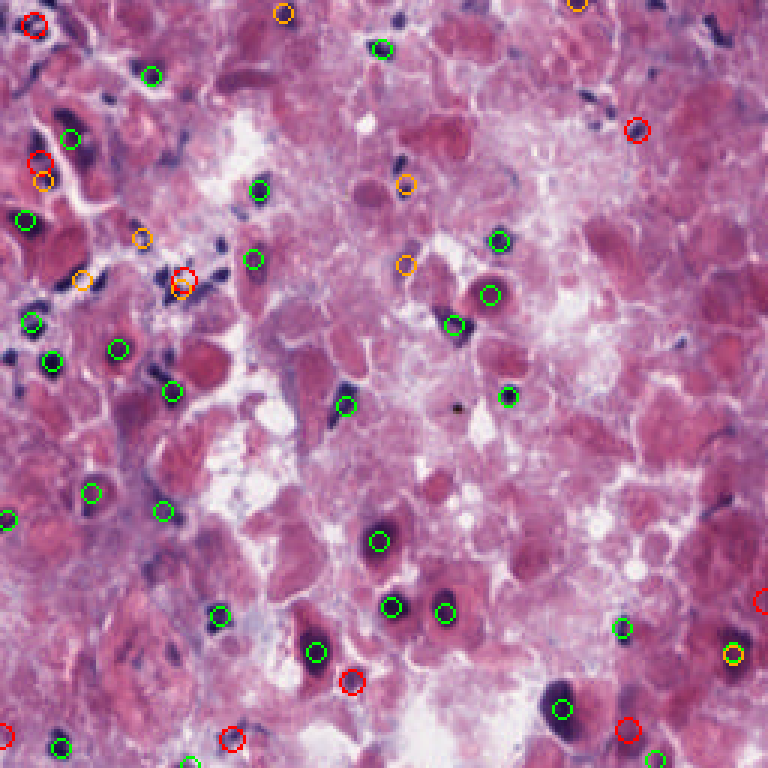
\includegraphics[width=.47\linewidth]{assets/casebook/p21_c_1025.png}\hfill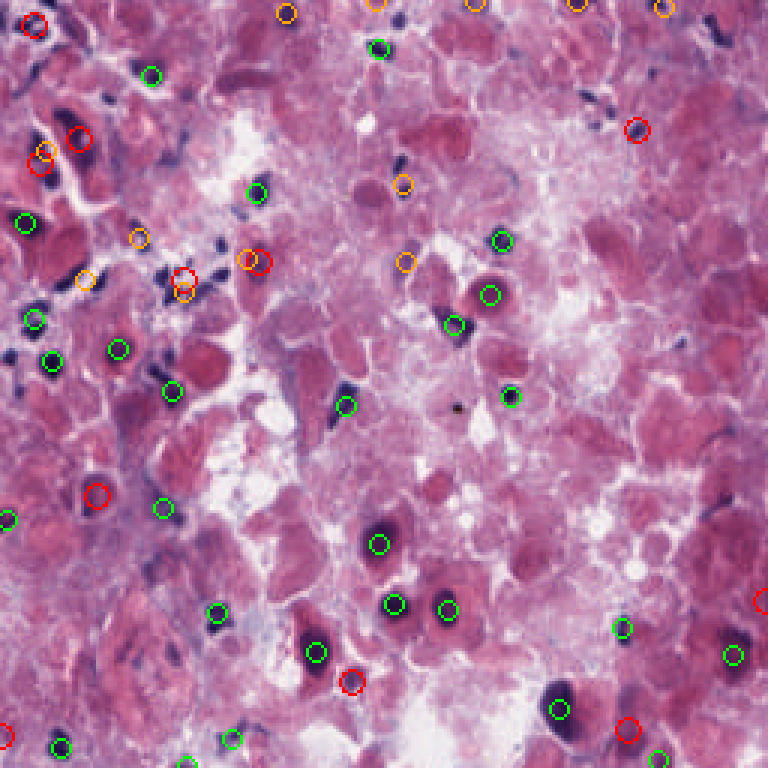
\includegraphics[width=.47\linewidth]{assets/casebook/p21_a_1025.png}\caption{P21编号1025的肺组织图像：左为对照方案，右为加入类别辅助任务的方案。绿色为成功找到的标注核，红色为漏检，橙色为多出的预测点。}\end{figure}
\section{P22：训练编码器全部24层后，找回了哪些细胞核？}
对照方案C训练预训练图像编码器的最后12层；方案M训练全部24层。种子19 死亡细胞核由67升至85，种子1由62升至82；总体检出率分别提高6.02和6.15个百分点，匹配精度提高3.64和3.46个百分点。种子19多产生488个候选，同时多匹配738个核，额外点减少250个；种子1分别为候选增加542、匹配增加753、额外点减少211。训练全部24层后，找到的细胞核增多，多余预测点减少。仅统计训练过程的耗时增加约42--43\%，峰值显存由4.05增至6.75 GiB。

145个死亡细胞核的逐对象对照给出更细的结果：种子19保留55个原有命中、新找到30个、丢失12个、两组均漏48个；种子1依次为56、26、6、57。种子19的肺组织图像净增12个、宫颈净增7个；结肠新增5个又丢失5个，净变化为0。面积小于67平方像素的死亡细胞核，在两个种子中均从7/32增至11/32。下面三张局部图把这些变化对应到具体核。

以下每组图从左到右依次为原始图像局部、对照方案的匹配结果和训练全部24层后的匹配结果。黑白双环标出同一个人工标注细胞核；绿色圆圈表示该标注核被找到，红色表示漏检，橙色表示多出的预测点。每幅局部图截取80×80原始像素并放大显示。图注中的预测分数，是模型中心预测图在标注中心周围3像素内的最高分数，取值范围为0到1；筛选阈值为0.5，后续还要经过峰值筛选和匹配。
\begin{figure}[H]\centering\begin{tikzpicture}
\begin{axis}[ybar,bar width=14pt,width=.9\linewidth,height=6cm,ymin=0,ymax=65,
 ylabel={\objectlabel},symbolic x coords={Retained,Gained,Lost,Missed},xtick=data,
 xticklabels={\retained,\gained,\lost,\missed},grid=major,nodes near coords,
 legend style={at={(.5,1.14)},anchor=north,legend columns=2}]
\addplot coordinates {(Retained,55) (Gained,30) (Lost,12) (Missed,48)};
\addplot coordinates {(Retained,56) (Gained,26) (Lost,6) (Missed,57)};
\legend{\seedname\ 19,\seedname\ 1}\end{axis}\end{tikzpicture}\caption{P22逐对象保留、新增、丢失和共同漏检。}\end{figure}
\begin{figure}[H]\centering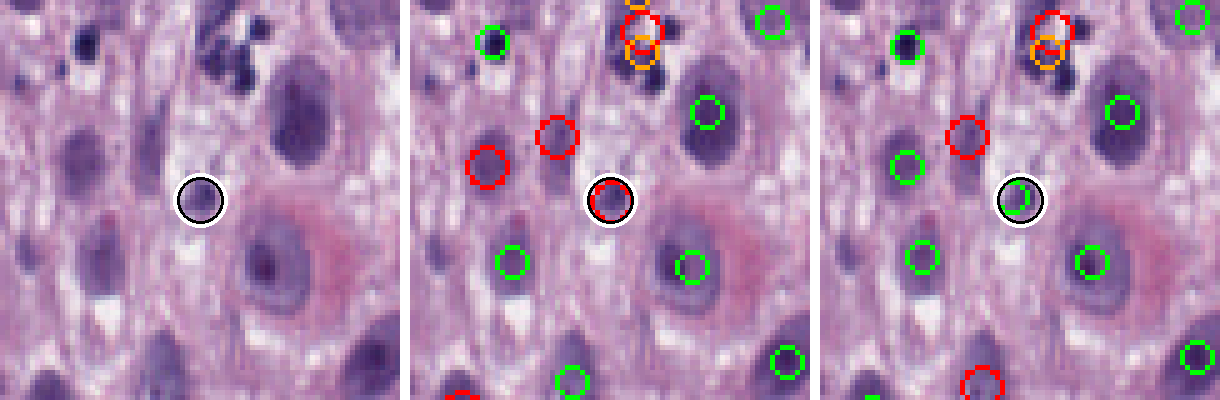
\includegraphics[width=.98\linewidth]{assets/casebook/recovered_1037.png}\caption{编号1037的肺组织图像，人工标注对象67（第98行、第180列，面积65平方像素）：对照方案的中心附近最高预测分数接近0，训练24层后升至0.792，该核从漏检变为成功匹配。}\end{figure}
该核较小，邻近深染结构。对照方案在这一位置的分数很低；训练24层后，模型在该位置找到一个与标注匹配的预测点。
\begin{figure}[H]\centering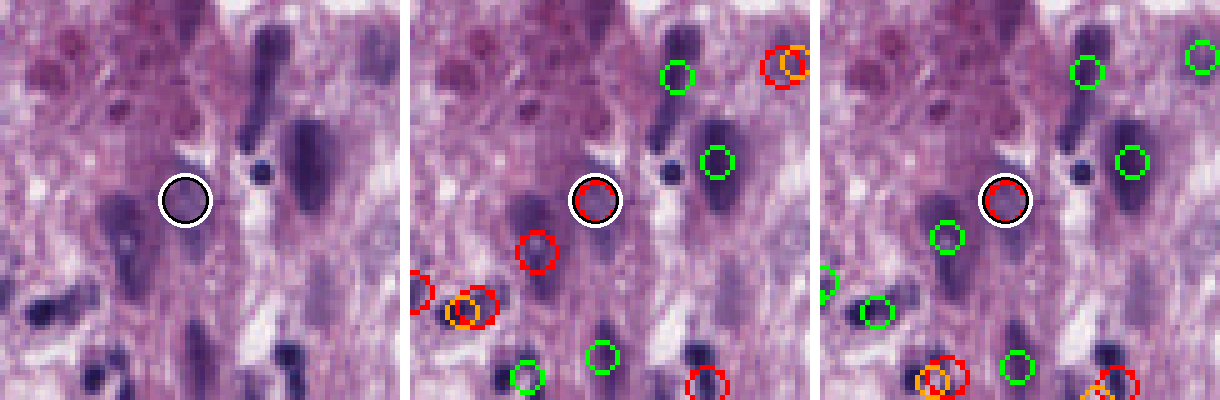
\includegraphics[width=.98\linewidth]{assets/casebook/missed_1037.png}\caption{编号1037的肺组织图像，人工标注对象57（第43行、第37列，面积214平方像素）：对照方案的最高预测分数接近0，训练24层后升至0.446；两个方案均漏检该核。}\end{figure}
该核周围有多个深染结构。训练24层后，中心附近的最高预测分数升高，但仍低于0.5，最终没有匹配到该核。
\begin{figure}[H]\centering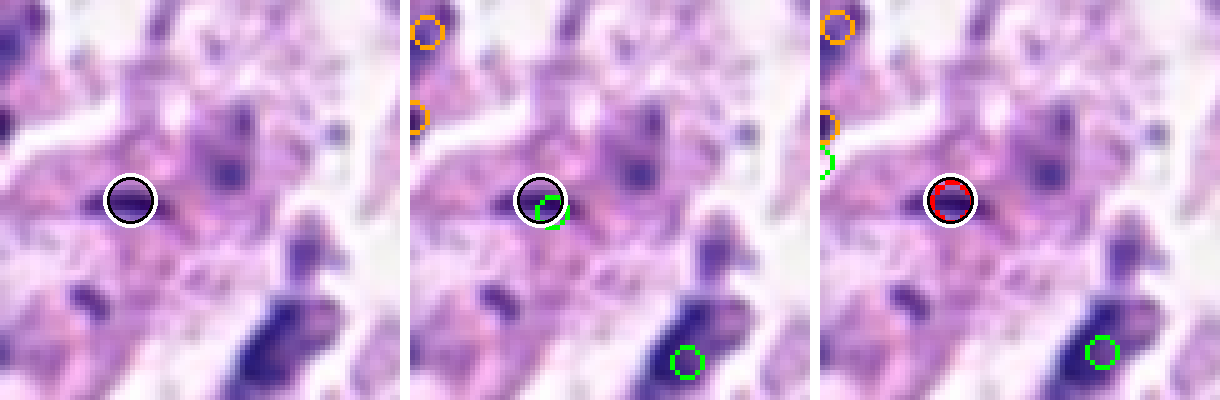
\includegraphics[width=.98\linewidth]{assets/casebook/lost_0776.png}\caption{编号776的结肠组织图像，人工标注对象7（第148行、第26列，面积137平方像素）：对照方案的最高预测分数为0.835并成功匹配；训练24层后分数为0.146，该核被漏检。}\end{figure}
这枚核在对照图中为绿色圆圈，在训练24层后的结果中为红圈。逐个比较人工标注的细胞核，可以同时看见新找回和丢失的对象。
\section{P23--P26：参数平均、学习率与预训练参数约束}
\subsection{P23：参数平均后，多数原有匹配得以保留}
每个随机种子训练一次，并分别使用最终模型参数C和指数移动平均后的参数E。指数移动平均给较近期的参数更大的权重，平均系数为0.999。死亡细胞核检出数由69到70、60到63；小型死亡细胞核在四个输出中均为6/32。种子19逐对象记录显示69个原命中全部保留，1个预测分数较低的细胞核变为匹配，72个的预测分数仍低于阈值。改善落在编号1025的肺组织图像的1个对象；种子1的增量分别落在结肠776、结肠1482和宫颈1756。使用平均参数后，多数原有匹配得以保留，小的死亡细胞核仍有较多漏检。

\subsection{P24：提高学习率后，不同图像中的结果}
编码器最后12层的学习率从 $10^{-5}$ 提至 $3\times10^{-5}$。两种子的匹配精度分别由0.688升至0.732、0.694升至0.731；候选减少589/471个，同时全体匹配增加29/38个。死亡细胞核分别由67升至78、68降至66。小型死亡细胞核均由7/32升至11/32；较大的死亡细胞核的变化分别为净增7、净减6，因此种子1的小核收益被其他对象的减少抵消。

编号1037的肺组织图像中死亡细胞核检出数在两种子分别增加5和3；同为肺组织图像的1025却分别减少1和3。编号1756的宫颈组织图像两个种子的变化为+2和-4。下图展示种子19的1037：右侧图中部分原红圈转为绿色，同时仍有红圈与橙圈；相邻核周围的响应变化各异。

\begin{figure}[H]\centering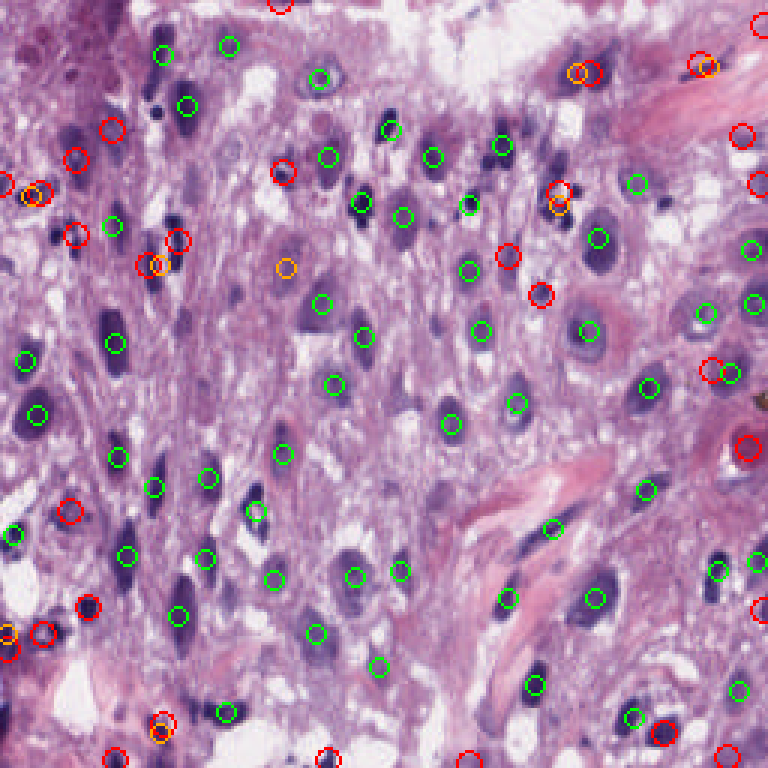
\includegraphics[width=.47\linewidth]{assets/casebook/p24_c_1037.png}\hfill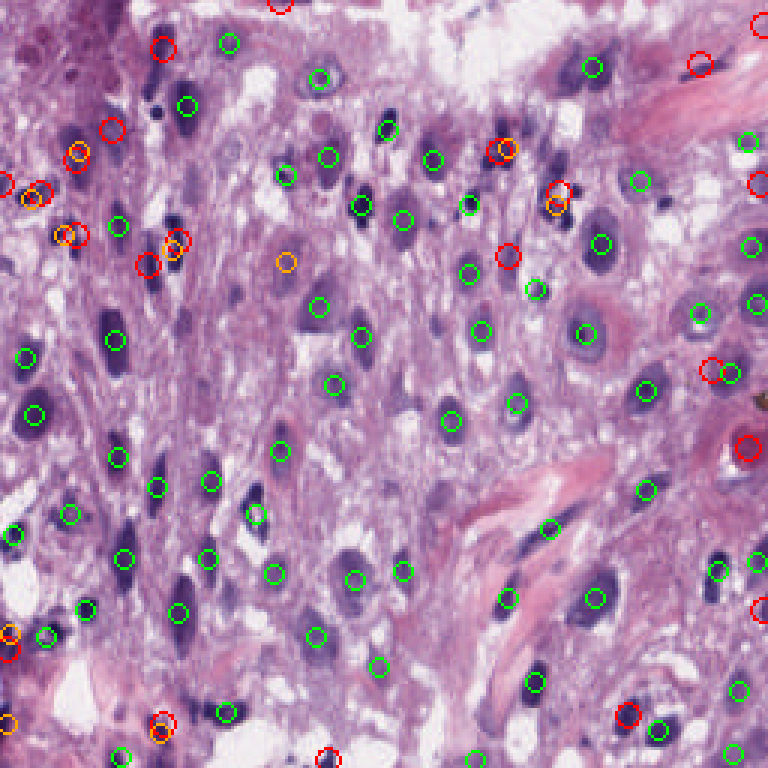
\includegraphics[width=.47\linewidth]{assets/casebook/p24_l_1037.png}\caption{P24编号1037的肺组织图像：左为对照方案，右为提高学习率后的方案，均为随机种子19。绿色为成功找到的标注核，红色为漏检，橙色为多出的预测点。}\end{figure}
\subsection{P25：分层设置学习率，提高总体检出率}
24层采用由低到高的分层学习率。两种子的总体检出率从0.590/0.598升至0.650/0.640，匹配精度从0.690/0.692升至0.744/0.742；死亡细胞核检出数从69到76、65到75。分别多匹配741和512个核，额外点减少510和544个。编号1037的肺组织图像由10到15、10到16，编号1482的结肠组织图像由15到9、14到10。肺组织和结肠组织中相反方向的变化，在两个种子的总体增量中均形成抵消。

\subsection{P26：约束编码器接近预训练参数}
P26在训练中增加约束，使编码器参数保持在预训练初始值附近。四项训练均完成130轮。种子19的死亡细胞核检出数从67到69，种子1从64到66；加入约束的方案R总体检出率为0.571/0.569，对照为0.584/0.596；方案R的匹配精度为0.679/0.688，对照为0.697/0.693。两个种子的配对死亡细胞核变化均为2/145，原始区间分别为 $[-0.006173,0.053793]$ 与 $[-0.071429,0.061224]$。这一约束对应较低的总体检出率和匹配精度，死亡细胞核检出数变化较小。

\section{综合分析：漏检发生在什么环节}
P22四个模型中，漏检的死亡细胞核有94.87\%--97.59\%在人工标注中心周围3像素内的最高预测分数低于0.5。种子19的对照方案和24层方案分别有74和57个这类细胞核；另有4和3个属于位置偏差或重复预测点筛选后的漏检。重复点筛选会保留附近较强的预测，减少同一位置的重复输出。对象57的分数虽升高仍低于阈值；对象67的分数升高后被成功找到；结肠对象7则出现分数下降。后续可在这些位置比较图像特征、训练集中形态相近的细胞核，以及不同组织中的预测分数。

本报告的配对数字均以同一轮、同一随机种子的对照方案计算；开发评估图像、人工标注对象和源文件见随附数值索引。\texttt{NUMBER\_SOURCES.md}给出数据路径、匹配定义和图像来源。
\begin{figure}[H]\centering\begin{tikzpicture}
\begin{axis}[ybar,bar width=9pt,width=.90\linewidth,height=7cm,ymin=0,ymax=.8,
 ylabel={\fractionlabel},symbolic x coords={C19,R19,C1,R1},xtick=data,grid=major,
 legend style={at={(.5,1.16)},anchor=north,legend columns=3}]
\addplot coordinates {(C19,.462069) (R19,.475862) (C1,.441379) (R1,.455172)};
\addplot coordinates {(C19,.583673) (R19,.570857) (C1,.596245) (R1,.569224)};
\addplot coordinates {(C19,.697221) (R19,.678537) (C1,.692519) (R1,.688080)};
\legend{\deadlabel,\overalllabel,\precisionlabel}
\end{axis}\end{tikzpicture}
\caption{P26四跑的死亡细胞核检出率、总体检出率和匹配精度。}\end{figure}
\end{document}
